\let\negmedspace\undefined
\let\negthickspace\undefined
\documentclass[journal]{IEEEtran}
\usepackage[a5paper, margin=10mm, onecolumn]{geometry}
%\usepackage{lmodern} % Ensure lmodern is loaded for pdflatex
\usepackage{tfrupee} % Include tfrupee package

\setlength{\headheight}{1cm} % Set the height of the header box
\setlength{\headsep}{0mm}     % Set the distance between the header box and the top of the text

\usepackage{gvv-book}
\usepackage{gvv}
\usepackage{cite}
\usepackage{amsmath,amssymb,amsfonts,amsthm}
\usepackage{algorithmic}
\usepackage{graphicx}
\usepackage{textcomp}
\usepackage{xcolor}
\usepackage{txfonts}
\usepackage{listings}
\usepackage{enumitem}
\usepackage{mathtools}
\usepackage{gensymb}
\usepackage{comment}
\usepackage[breaklinks=true]{hyperref}
\usepackage{tkz-euclide} 
\usepackage{listings}
% \usepackage{gvv}                                        
\def\inputGnumericTable{}                                 
\usepackage[latin1]{inputenc}                                
\usepackage{color}                                            
\usepackage{array}                                            
\usepackage{longtable}                                       
\usepackage{calc}                                             
\usepackage{multirow}                                         
\usepackage{hhline}                                           
\usepackage{ifthen}                                           
\usepackage{lscape}
\begin{document}

\bibliographystyle{IEEEtran}
\vspace{3cm}

\title{1-1.4-9n}
\author{EE24BTECH11022 - Eshan Sharma
}
% \maketitle
% \newpage
% \bigskip
{\let\newpage\relax\maketitle}

\renewcommand{\thefigure}{\theenumi}
\renewcommand{\thetable}{\theenumi}
\setlength{\intextsep}{10pt} % Space between text and floats


\numberwithin{equation}{enumi}
\numberwithin{figure}{enumi}
\renewcommand{\thetable}{\theenumi}


\textbf{Question}:\\
Consider two points $\vec{P}$ and $\vec{Q}$ with position vectors $\overrightarrow{OP} = \overrightarrow{3a} - \overrightarrow{2b}$ and $\overrightarrow{OQ} = \overrightarrow{a} + \overrightarrow{b}$. Find the position vector of a point $\vec{R}$ which divides the line joining $\vec{P}$ and $\vec{Q}$ in the ratio 2 : 1, \\ 
i) internally, and \\
ii) externally
\\
\textbf{Solution:}\\
Using Section formula, \\
i) For internal,\\
\begin{align*}
\overrightarrow{OP} &= 3\overrightarrow{a} - 2\overrightarrow{b} \\
\overrightarrow{OQ} &= \overrightarrow{a} + \overrightarrow{b} \\
\overrightarrow{OR} &= \frac{1 \times \overrightarrow{OP} + 2 \times \overrightarrow{OQ}}{3} \\
\overrightarrow{OR} &= \frac{1 \times (3\overrightarrow{a} - 2\overrightarrow{b}) + 2 \times (\overrightarrow{a} + \overrightarrow{b})}{3} \\
\overrightarrow{OR} &= \frac{3\overrightarrow{a} - 2\overrightarrow{b} + 2\overrightarrow{a} + 2\overrightarrow{b}}{3} \\
\overrightarrow{OR} &= \frac{5\overrightarrow{a}}{3}
\end{align*}

ii) For external,\\
\begin{align*}
\overrightarrow{OP} &= 3\overrightarrow{a} - 2\overrightarrow{b} \\
\overrightarrow{OQ} &= \overrightarrow{a} + \overrightarrow{b} \\
\overrightarrow{OR} &= \frac{2 \times \overrightarrow{OQ} - 1 \times \overrightarrow{OP}}{2 - 1} \\
\overrightarrow{OR} &= \frac{2 \times (\overrightarrow{a} + \overrightarrow{b}) - 1 \times (3\overrightarrow{a} - 2\overrightarrow{b})}{1} \\
\overrightarrow{OR} &= \frac{2\overrightarrow{a} + 2\overrightarrow{b} - 3\overrightarrow{a} + 2\overrightarrow{b}}{1} \\
\overrightarrow{OR} &= \overrightarrow{-a} + 4\overrightarrow{b}
\end{align*}

\begin{figure}[ht]
   \centering
   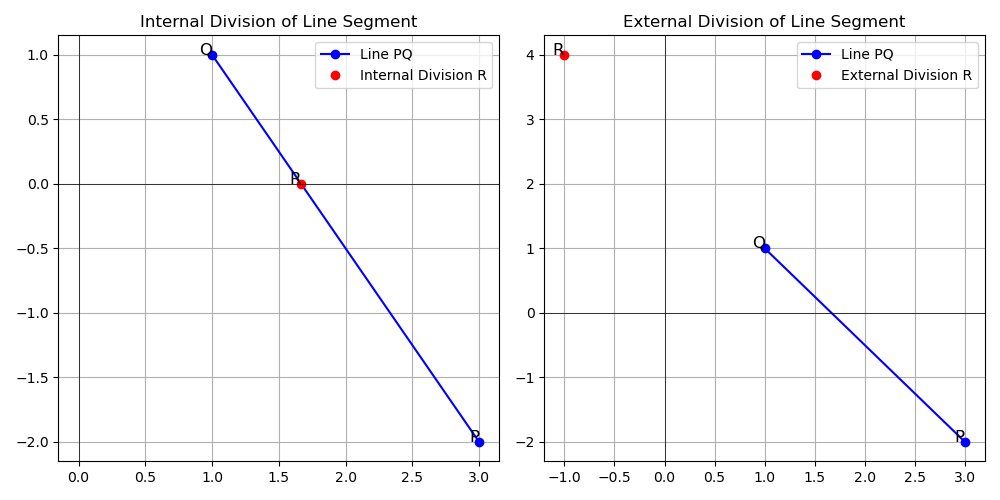
\includegraphics[width=0.7\linewidth]{figs/1-1.4-9n.png}
   \caption{Plot of $\overrightarrow{OR}$ in internal and external division}
   \label{fig:1}
\end{figure}


\end{document}  
\end{document}
